\chapter{Propuesta de solución}
\label{chap:chapter2}

El presente capítulo expone la propuesta de solución del videojuego educativo \textit{Go Goals! Digital}, detallando las decisiones técnicas y metodológicas que sustentan su concepción e implementación. Se estructura en tres ejes principales guiados por la metodología Extreme Programming. El primero es la planificación, donde se definen los requisitos y la organización iterativa del proyecto. El segundo es el diseño, que abarca la arquitectura del sistema, los prototipos de interfaces y las tarjetas CRC. El tercero es la implementación, que describe los estándares de codificación, los patrones de diseño aplicados y las tareas de ingeniería ejecutadas. A través de este recorrido, se proporciona una visión sistemática de cómo se materializó la solución, respaldada por tablas, modelos y diagramas que garantizan la calidad y coherencia del producto.

%---------------------------------------------------------------------------
\section{Descripción de la propuesta de solución}
\label{sec:descripcion_propuesta}

\textit{Go Goals! Digital} es un videojuego educativo basado en la adaptación digital del juego de mesa oficial \textit{Go Goals!} de las Naciones Unidas \parencite{GoGoals2020}. En su formato digital, los jugadores, de uno a cuatro participantes, controlan fichas en un tablero hexagonal de 63 casillas que metaforiza el recorrido colectivo hacia el año 2030, horizonte establecido por la Agenda 2030 para el Desarrollo Sostenible \parencite{NacionesUnidas2015}. El avance se determina mediante un dado virtual, y al caer en una de las 17 casillas temáticas, distribuidas equitativamente una por cada ODS, el jugador debe responder una pregunta de opción múltiple sobre el objetivo correspondiente. Las respuestas correctas activan el efecto de escalera para un avance positivo, mientras que las incorrectas activan el efecto de serpiente para un retroceso correctivo, preservando la mecánica pedagógica central del juego original.

Las principales mejoras que introduce la versión digital respecto al formato físico son:
\begin{itemize}
    \item \textbf{Accesibilidad universal}: exportación nativa a plataformas de escritorio como Windows, Linux y macOS, sin necesidad de materiales físicos ni impresión.
    \item \textbf{Contenido dinámico}: banco de preguntas ampliable en formato JSON, editable por educadores sin conocimientos de programación.
    \item \textbf{Retroalimentación enriquecida}: animaciones de fichas, efectos de sonido y retroalimentación visual inmediata a través de colores y partículas al responder.
    \item \textbf{Seguimiento del aprendizaje}: registro automático de respuestas correctas e incorrectas por jugador y por ODS.
    \item \textbf{Rejugabilidad}: selección aleatoria y sin repetición de preguntas dentro de cada sesión, evitando la memorización.
\end{itemize}

\begin{figure}[H]
  \centering
  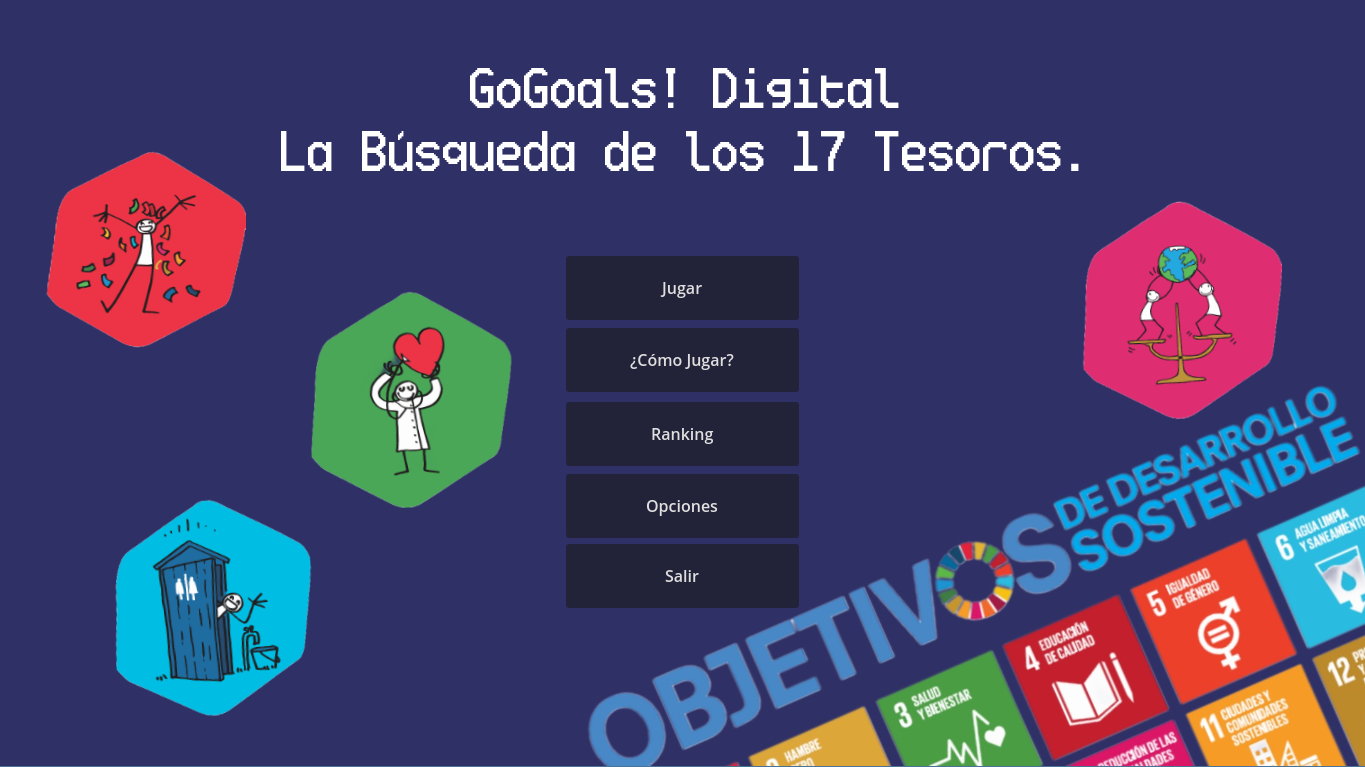
\includegraphics[width=0.85\textwidth]{Images/Menú Principal}
  \caption{Vista general del videojuego educativo \textit{Go Goals! Digital} (elaboración propia).\label{fig:propuesta_solucion}}
\end{figure}

Dentro del ecosistema de recursos educativos digitales sobre desarrollo sostenible, \textit{Go Goals! Digital} ocupa un nicho específico: es el único videojuego desarrollado en Cuba que adapta fielmente la mecánica del juego de mesa oficial de las Naciones Unidas a un entorno digital interactivo. A diferencia de otras iniciativas educativas basadas en vídeos o materiales estáticos, este videojuego integra la competencia entre varios jugadores, el azar controlado y la evaluación del conocimiento en una sola experiencia lúdica. La plataforma Godot Engine, elegida por su licencia libre MIT y su capacidad de exportación multiplataforma, garantiza la ejecución nativa en sistemas operativos de escritorio tales como Windows, Linux y macOS sin requerir configuraciones complejas, lo que resulta especialmente relevante en contextos educativos con recursos tecnológicos limitados.

El diseño del videojuego respeta los colores, íconos y denominaciones oficiales de cada ODS, lo que refuerza la identificación visual del contenido educativo y facilita su uso como complemento de programas curriculares relacionados con la sostenibilidad.

%---------------------------------------------------------------------------
\section{Planificación}
\label{sec:planificacion}

El presente epígrafe se enfoca en la organización y gestión del proyecto siguiendo la metodología Extreme Programming (XP). La planificación en XP se centra en la flexibilidad y la colaboración continua con el cliente, utilizando iteraciones cortas para adaptarse a cambios y priorizar funcionalidades \parencite{Beck2004}. Aquí se detallan los procesos clave que guían el desarrollo de \textit{Go Goals! Digital}, desde la obtención de requisitos hasta la definición de historias de usuario, la estimación de tiempo y el plan de iteraciones.

Como parte inicial de esta planificación, se realizaron sesiones de tormenta de ideas con el cliente para enfocar el proyecto en la arquitectura general, y posteriormente se llevaron a cabo reuniones que resultaron en la definición de los requisitos funcionales, no funcionales e historias de usuario.

\subsection{Requisitos funcionales}
\label{subsec:req_funcionales}

Los requisitos funcionales constituyen el conjunto de capacidades, comportamientos y procesos que un sistema debe implementar para satisfacer las necesidades de sus usuarios. Definen de manera precisa y verificable qué debe hacer el sistema: las entradas que procesa, las transformaciones que aplica y las salidas que produce \parencite{Sommerville2021, Pressman2019}. Para \textit{Go Goals! Digital}, los requisitos se obtuvieron mediante sesiones de trabajo con el cliente y el análisis de las mecánicas del juego de mesa original, priorizando las funcionalidades esenciales para la experiencia educativa.

\begin{longtable}{|c|p{0.3\textwidth}|p{0.37\textwidth}|c|c|}
\caption{Requisitos funcionales del videojuego Go Goals! Digital (elaboración propia).\label{tab:req_funcionales}} \\
\hline
\textbf{ID} & \textbf{Nombre} & \textbf{Descripción} & \textbf{Prioridad} & \textbf{Complejidad} \\
\hline
\endfirsthead
\multicolumn{5}{c}
{{ \tablename\ \thetable{} -- Continuación de la página anterior}} \\
\hline
\textbf{ID} & \textbf{Nombre} & \textbf{Descripción} & \textbf{Prioridad} & \textbf{Complejidad} \\
\hline
\endhead
\hline
RF-01 & Mostrar menú principal & El sistema debe contar con un menú principal con opciones de iniciar partida, ver instrucciones y salir. & Alta & Baja \\
\hline
RF-02 & Mostrar pantalla de instrucciones & El sistema debe mostrar las reglas del juego de manera clara y accesible. & Media & Baja \\
\hline
RF-03 & Iniciar partida & El sistema debe permitir al usuario iniciar una nueva partida configurando el número de jugadores hasta 4. & Alta & Baja \\
\hline
RF-04 & Visualizar tablero & El sistema debe mostrar el tablero hexagonal completo con las 63 casillas correctamente identificadas. & Alta & Media \\
\hline
RF-05 & Lanzar dado & El sistema debe simular el lanzamiento de un dado de 6 caras con resultado pseudoaleatorio. & Alta & Baja \\
\hline
RF-06 & Mover ficha & El sistema debe mover la ficha del jugador activo la cantidad de casillas indicada por el dado con animación. & Alta & Media \\
\hline
RF-07 & Aplicar efecto de escalera & El sistema debe detectar casillas de escalera y aplicar el avance correspondiente con animación. & Alta & Media \\
\hline
RF-08 & Aplicar efecto de serpiente & El sistema debe detectar casillas de serpiente y aplicar el retroceso correspondiente con animación. & Alta & Media \\
\hline
RF-09 & Mostrar pregunta ODS & El sistema debe mostrar una pregunta aleatoria del banco cuando una ficha cae en casilla temática. & Alta & Alta \\
\hline
RF-10 & Evaluar respuesta & El sistema debe evaluar la respuesta del jugador, mostrar retroalimentación y aplicar el efecto correspondiente. & Alta & Media \\
\hline
RF-11 & Gestionar turnos & El sistema debe gestionar el turno de cada jugador de forma automática y mostrar el jugador activo. & Alta & Media \\
\hline
RF-12 & Determinar condición de victoria & El sistema debe detectar cuando un jugador llega a la casilla 63 y mostrar la pantalla de victoria. & Alta & Baja \\
\hline
RF-13 & Mostrar estadísticas de partida & El sistema debe registrar y mostrar las respuestas correctas e incorrectas por jugador y por ODS. & Media & Alta \\
\hline
RF-14 & Configurar audio & El sistema debe permitir activar o desactivar música y efectos de sonido. & Baja & Baja \\
\hline
RF-15 & Pausar partida & El sistema debe permitir pausar la partida en cualquier momento y reanudarla desde el mismo estado. & Media & Baja \\
\hline
RF-16 & Reiniciar partida & El sistema debe permitir reiniciar la partida actual desde el inicio sin volver al menú principal. & Media & Baja \\
\hline
RF-17 & Habilitar cámara de seguimiento & El sistema debe incluir una cámara dinámica que enfoque automáticamente al jugador activo durante su turno. & Baja & Media \\
\hline
RF-18 & Habilitar modo de práctica & El sistema debe permitir al usuario jugar en solitario para recorrer el tablero, practicar y familiarizarse con el juego. & Media & Baja \\
\hline
\hline
\end{longtable}

\subsection{Requisitos no funcionales}
\label{subsec:req_no_funcionales}

Los requisitos no funcionales son aquellas especificaciones que describen cómo debe ser un sistema en términos de atributos de calidad, como rendimiento, seguridad, usabilidad y escalabilidad, en lugar de simplemente describir sus funciones. Estos requisitos se centran en aspectos como la eficiencia, confiabilidad y facilidad de mantenimiento del sistema, que son fundamentales para garantizar su éxito y aceptación por parte de los usuarios. Al considerar los requisitos no funcionales desde las etapas iniciales del desarrollo de software, se puede diseñar un sistema que cumpla con las expectativas de los usuarios en términos de calidad y experiencia de uso \parencite{Pressman2019}.

\textbf{Requisitos no funcionales de Usabilidad}

RNF-01: El sistema debe ser intuitivo y de fácil comprensión para usuarios de todas las edades.

RNF-02: Todos los textos de la interfaz deben renderizarse con una tipografía de tamaño igual o superior a 16pt para garantizar legibilidad.

RNF-03: Los botones interactivos principales deben poseer un área de colisión amplia y holgada para facilitar la interacción en pantallas táctiles y el acceso motriz.

RNF-04: La paleta de colores debe mantener un contraste alto entre el texto y el fondo, respetando los colores e íconos oficiales de los 17 ODS de las Naciones Unidas.

RNF-05: Al presentarse una funcionalidad nueva en la partida, el sistema debe mostrar una indicación o tutorial contextual breve.

\textbf{Requisitos no funcionales de Rendimiento}

RNF-06: El sistema debe responder a acciones del usuario, tales como lanzar el dado o seleccionar una respuesta, en menos de 0{,}5 segundos en hardware de gama media.

RNF-07: El ejecutable para Windows no debe superar los 150~MB para facilitar su distribución en contextos con ancho de banda limitado.

\textbf{Requisitos no funcionales de Software}

RNF-08: El videojuego debe ser compatible con Windows 10+, Linux (Ubuntu 20.04+) y macOS 11+.

RNF-09: La versión de escritorio debe funcionar completamente sin conexión a internet (disponibilidad offline).

RNF-10: El código GDScript debe mantener comentarios de documentación internos en todas las clases para garantizar la mantenibilidad.

\textbf{Requisitos no funcionales de Hardware}

RNF-11: El dispositivo debe poseer un procesador de doble núcleo a 1{,}5~GHz o superior.

RNF-12: El sistema debe contar con al menos 512~MB de memoria RAM disponible para la ejecución del videojuego.

RNF-13: Se debe disponer de al menos 300~MB de espacio libre en la unidad de almacenamiento para la instalación del ejecutable y sus archivos de datos.

\subsection{Historias de usuario}
\label{subsec:historias_usuario}

Las historias de usuario son una técnica fundamental en metodologías ágiles como Extreme Programming (XP), utilizadas para capturar requisitos desde la perspectiva del usuario final. Según \citeauthor{Cohn2005} \parencite{Cohn2005}, una historia de usuario es ``una descripción breve y simple de una funcionalidad deseada, expresada en lenguaje cotidiano y centrada en el valor que aporta al usuario''. A diferencia de los documentos de requisitos tradicionales, las historias de usuario son más flexibles, pero siguen el formato estandarizado:

\begin{center}
\textit{``Como [rol], quiero [acción], para [beneficio]''}
\end{center}

A continuación se presenta, a modo representativo, la historia de usuario más destacada del videojuego por su relevancia en la asimilación del contenido (Tabla \ref{tab:hu9}). El conjunto completo de dieciocho historias de usuario que componen el \textit{Product Backlog} se encuentra listado en el Anexo \ref{anx:historias_usuario}.

\begin{table}[H]
\centering
\caption{Historia de usuario 9: Mostrar pregunta ODS (elaboración propia).\label{tab:hu9}}
\renewcommand{\arraystretch}{1.5}
\begin{tabular}{|p{0.45\textwidth}|p{0.45\textwidth}|}
\hline
\multicolumn{2}{|l|}{\textbf{Historia de Usuario}} \\
\hline
\textbf{Número:} 9 & \textbf{Nombre:} Mostrar pregunta ODS \\
\hline
\textbf{Prioridad:} Alta & \textbf{Riesgo:} Alto \\
\hline
\textbf{Puntos de estimación:} 5.0 & \textbf{Iteración asignada:} 3 \\
\hline
\multicolumn{2}{|p{0.945\textwidth}|}{\textbf{Descripción:} Como jugador quiero responder preguntas cuando caiga en una casilla temática de ODS para aprender interactivamente sobre la sostenibilidad.} \\
\hline
\multicolumn{2}{|p{0.945\textwidth}|}{\textbf{Observaciones:}
\vspace{-0.5em}
\begin{itemize}
    \setlength\itemsep{0em}
    \item El juego debe pausar el turno al caer en casilla temática.
    \item Se debe mostrar un panel modal con el ícono del ODS, el texto de la pregunta y las opciones de respuesta.
    \item Se selecciona una pregunta aleatoria sin repetir dentro de la sesión.
\end{itemize}
\vspace{-1em}
} \\
\hline
\end{tabular}
\end{table}

\subsection{Estimación de tiempo de desarrollo}
\label{subsec:estimacion}

Los puntos de estimación en el desarrollo ágil se utilizan para medir el esfuerzo relativo requerido para completar una historia de usuario, en lugar de estimar el tiempo exacto. Esto sirve para evaluar su complejidad, comparar historias de usuario y planificar las iteraciones \parencite{Cohn2005}.

\begin{longtable}{|c|p{0.45\textwidth}|c|}
\caption{Puntos de estimación por historia de usuario (elaboración propia).\label{tab:estimacion}} \\
\hline
\textbf{No. HU} & \textbf{Nombre} & \textbf{Puntos (días)} \\
\hline
\endfirsthead
\multicolumn{3}{c}%
{{\tablename\ \thetable{} -- Continuación de la página anterior}} \\
\hline
\textbf{No. HU} & \textbf{Nombre} & \textbf{Puntos (días)} \\
\hline
\endhead
\hline
\endfoot
\hline
\endlastfoot
1. & Mostrar menú principal & 1.0 \\
\hline
2. & Mostrar pantalla de instrucciones & 1.0 \\
\hline
3. & Iniciar partida & 2.0 \\
\hline
4. & Visualizar tablero & 5.0 \\
\hline
5. & Lanzar dado & 1.5 \\
\hline
6. & Mover ficha & 4.0 \\
\hline
7. & Aplicar efecto de escalera & 1.5 \\
\hline
8. & Aplicar efecto de serpiente & 1.5 \\
\hline
9. & Mostrar pregunta ODS & 5.0 \\
\hline
10. & Evaluar respuesta & 3.0 \\
\hline
11. & Gestionar turnos & 2.0 \\
\hline
12. & Determinar condición de victoria & 1.5 \\
\hline
13. & Mostrar estadísticas de partida & 4.0 \\
\hline
14. & Configurar audio & 2.5 \\
\hline
15. & Pausar partida & 1.0 \\
\hline
16. & Reiniciar partida & 1.0 \\
\hline
17. & Habilitar cámara de seguimiento & 2.0 \\
\hline
18. & Habilitar modo de práctica & 5.0 \\
\hline
\multicolumn{2}{|r|}{\textbf{Total}} & \textbf{44.5} \\
\hline
\end{longtable}

\subsection{Plan de iteraciones}
\label{subsec:plan_iteraciones}

El plan de iteraciones es una herramienta esencial para organizar y coordinar el trabajo del equipo de desarrollo siguiendo la metodología Extreme Programming. Cada iteración se planifica con una duración de una a tres semanas y comienza con una reunión de planificación en la que el cliente presenta las historias de usuario priorizadas, y el equipo de desarrollo estima y se compromete a completar las tareas necesarias \parencite{Cohn2005}. Al finalizar cada iteración, se entrega un incremento funcional del software que puede ser evaluado por el cliente, cerrando el ciclo de retroalimentación y permitiendo ajustar las prioridades para la iteración siguiente \parencite{Beck2004}.

Para \textit{Go Goals! Digital}, el desarrollo se organizó en cinco iteraciones que siguen una progresión lógica: las dos primeras sientan las bases del proyecto; la tercera integra el núcleo pedagógico; la cuarta incorpora funcionalidades de cierre y configuración; y la quinta agrega características complementarias que mejoran la experiencia de usuario. Esta estructura permite validar tempranamente las funcionalidades de mayor riesgo técnico, como la visualización del tablero hexagonal y el motor de preguntas, antes de proceder con los componentes de menor complejidad.

\begin{longtable}{|c|c|p{0.45\textwidth}|c|}
\caption{Plan de iteraciones de desarrollo (elaboración propia).\label{tab:plan_iteraciones}} \\
\hline
\textbf{Iteración} & \textbf{No. HU} & \textbf{Historia de Usuario} & \textbf{Duración (días)} \\
\hline
\endfirsthead
\multicolumn{4}{c}%
{{\tablename\ \thetable{} -- Continuación de la página anterior}} \\
\hline
\textbf{Iteración} & \textbf{No. HU} & \textbf{Historia de Usuario} & \textbf{Duración (días)} \\
\hline
\endhead
\hline
\endfoot
\hline
\endlastfoot
\multirow{4}{*}{1} & 1 & Mostrar menú principal & \multirow{4}{*}{9.0} \\
\cline{2-3}
 & 2 & Mostrar pantalla de instrucciones & \\
\cline{2-3}
 & 3 & Iniciar partida & \\
\cline{2-3}
 & 4 & Visualizar tablero & \\
\hline
\multirow{4}{*}{2} & 5 & Lanzar dado & \multirow{4}{*}{8.5} \\
\cline{2-3}
 & 6 & Mover ficha & \\
\cline{2-3}
 & 7 & Aplicar efecto de escalera & \\
\cline{2-3}
 & 8 & Aplicar efecto de serpiente & \\
\hline
\multirow{3}{*}{3} & 9 & Mostrar pregunta ODS & \multirow{3}{*}{10.0} \\
\cline{2-3}
 & 10 & Evaluar respuesta & \\
\cline{2-3}
 & 11 & Gestionar turnos & \\
\hline
\multirow{5}{*}{4} & 12 & Determinar condición de victoria & \multirow{5}{*}{10.0} \\
\cline{2-3}
 & 13 & Mostrar estadísticas de partida & \\
\cline{2-3}
 & 14 & Configurar audio & \\
\cline{2-3}
 & 15 & Pausar partida & \\
\cline{2-3}
 & 16 & Reiniciar partida & \\
\hline
\multirow{2}{*}{5} & 17 & Habilitar cámara de seguimiento & \multirow{2}{*}{7.0} \\
\cline{2-3}
 & 18 & Habilitar modo de práctica & \\
\hline
\multicolumn{3}{|r|}{\textbf{Total}} & \textbf{44.5} \\
\hline
\end{longtable}

%---------------------------------------------------------------------------
\section{Diseño}
\label{sec:diseno}

El presente epígrafe constituye la transición esencial entre la planificación teórica y la implementación práctica, donde se materializan los requisitos en soluciones técnicas concretas. Este apartado se centra en tres pilares fundamentales: la arquitectura del sistema, que detalla cómo la estructura basada en nodos y el SceneTree de Godot permiten organizar los componentes clave del videojuego; los prototipos de interfaces gráficas de usuario; y las tarjetas CRC que definen la interacción entre las clases del sistema.

\subsection{Arquitectura Jerárquica Basada en Nodos}
\label{subsec:arquitectura}

Godot Engine utiliza una arquitectura jerárquica basada en nodos, la cual es identificada como el árbol de escenas. En esta arquitectura, los \textbf{nodos} son los bloques de construcción fundamentales: cada elemento del videojuego, desde una ficha de jugador hasta un efecto de sonido, es un nodo que hereda de la clase base \texttt{Node}. Los nodos se organizan en \textbf{escenas}, que son composiciones reutilizables de nodos agrupados jerárquicamente; una escena puede representar desde un botón hasta una pantalla completa del juego. El \textbf{SceneTree} es la estructura global que gestiona todas las escenas y nodos en tiempo de ejecución, funcionando como un árbol de procesamiento que organiza el orden de ejecución de métodos, la jerarquía de transformaciones y la gestión de señales que comunican a los nodos entre sí \parencite{GodotDocs2026}.

El uso del SceneTree aporta ventajas significativas para \textit{Go Goals! Digital}. En primer lugar, aumenta la modularidad al permitir tener una escena para cada funcionalidad específica, como podría ser una ficha de jugador, que puede instanciarse dentro de otra escena más grande como el tablero. De esta manera, el tablero puede contener varias fichas, cada una con sus propiedades individuales (color, posición, nombre del jugador). Al momento de necesitar cambiarlas todas, se pueden realizar modificaciones en la escena de la ficha, reflejándose automáticamente en todas las instancias. Otra ventaja es el rendimiento, que mejora debido a que evita actualizaciones innecesarias y permite operaciones masivas como llamadas de métodos en grupos de nodos. Su diseño trae un enfoque de composición sobre herencia para no depender de jerarquías rígidas de clases y posee funcionalidades para realizar cambios de escenas de forma fluida.

La comunicación entre estos elementos se simplifica gracias al sistema de señales integrado, permitiendo que eventos como el lanzamiento del dado, el movimiento de fichas o la presentación de preguntas se coordinen eficientemente sin acoplamiento rígido entre componentes. Además, el SceneTree optimiza automáticamente el rendimiento al gestionar el orden de procesamiento y renderizado, algo relevante en un juego de tablero donde múltiples fichas, animaciones y elementos de interfaz pueden interactuar simultáneamente en pantalla. La capacidad de pausar o manipular selectivamente ramas enteras del árbol de escenas es particularmente útil para implementar mecánicas como el menú de pausa o la transición entre el tablero y el panel de preguntas educativas.

\begin{figure}[!htbp]
  \centering
  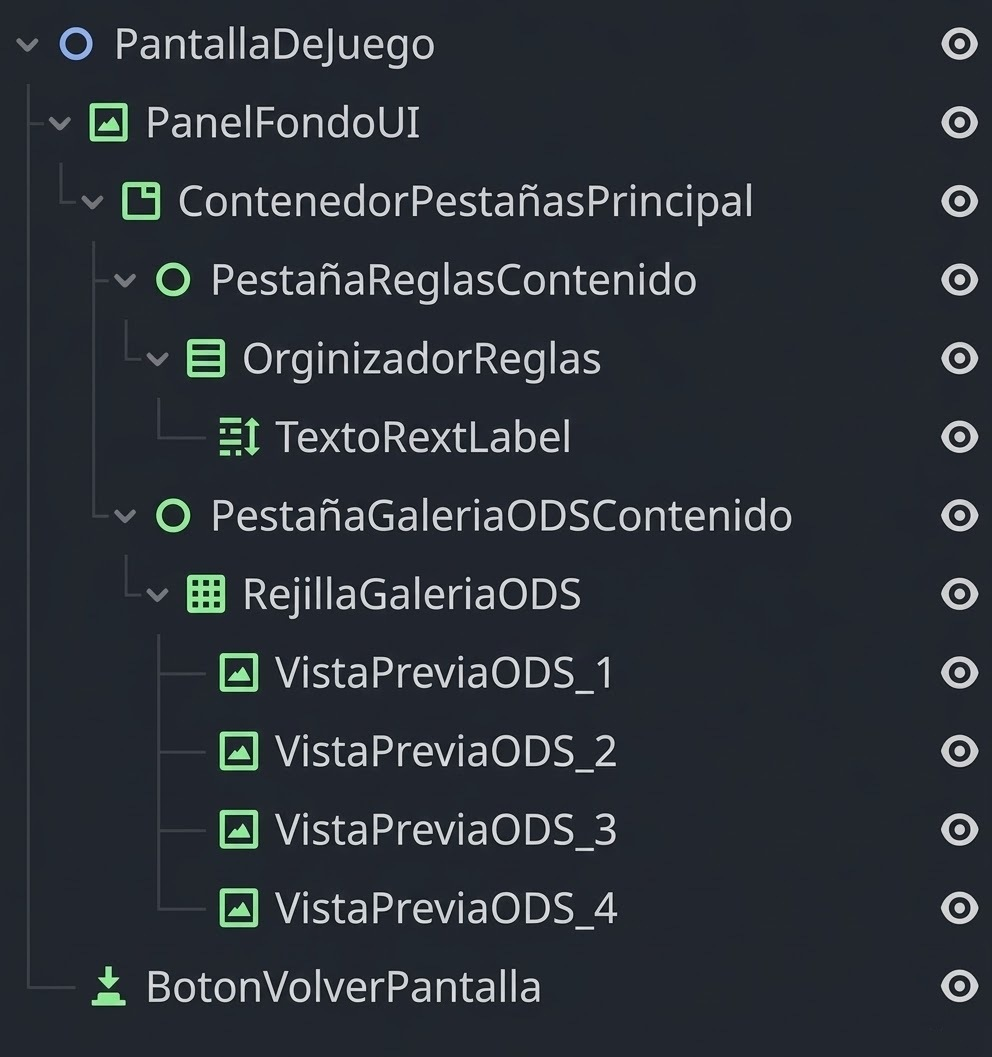
\includegraphics[width=0.55\textwidth]{Images/SceeneTree}
  \caption{Ejemplo de jerarquía de nodos en el SceneTree de Godot: pantalla de instrucciones del videojuego \textit{Go Goals! Digital} (elaboración propia).\label{fig:scene_tree}}
\end{figure}

El videojuego \textit{Go Goals! Digital} emplea esta Arquitectura Jerárquica Basada en Nodos, apoyada por servicios globales y coordinada centralmente. Esta elección arquitectural no es arbitraria: frente a alternativas como un patrón \textit{Model-View-Controller} clásico o una separación por capas estricta, la composición de nodos de Godot resulta superior para este proyecto por razones concretas de extensibilidad y mantenibilidad. Un MVC rígido tendería a concentrar en el controlador una cantidad creciente de lógica de presentación a medida que se incorporen nuevas mecánicas, como nuevos tipos de casillas o modos de juego, generando un acoplamiento progresivo entre la vista y el controlador. La composición orientada a nodos, en cambio, permite agregar una nueva funcionalidad como un nodo hijo con su propio script, sin tocar el controlador principal. Esto favorece directamente la extensibilidad y reduce el riesgo de regresiones al modificar el sistema. Como buena práctica de diseño, se estructuró el proyecto en cuatro pilares fundamentales de responsabilidad:

\begin{itemize}
    \item \textbf{Arquitectura Orientada a Escenas}: La navegación principal y los límites de las interfaces dependen del sistema nativo de escenas de Godot. Entornos como el menú principal, la pantalla de juego interactiva y el menú de fin de partida funcionan como fronteras naturales de presentación. Dentro del juego, el nivel principal actúa como controlador de composición local, ensamblando las dependencias y conectando la interfaz de usuario con la lógica sin mezclar directamente sus responsabilidades.
    
    \item \textbf{Servicios Globales y Autoloads}: Godot facilita el patrón Singleton a través de nodos que se registran globalmente, permitiendo el acceso a funcionalidades transversales desde cualquier escena. El proyecto emplea la clase \texttt{GameData} para mantener la configuración de la partida y cargar el banco de preguntas; \texttt{AudioManager} para centralizar la reproducción de música y efectos de sonido; y \texttt{RecordsManager} para gestionar la persistencia local de las puntuaciones de forma estructurada e independiente.
    
    \item \textbf{Coordinación Central y Comunicación por Eventos}: El flujo del juego es orquestado por el coordinador central \texttt{GameManager}. Este componente concentra los casos de uso principales, como el control de turnos, el movimiento, las preguntas y la victoria. La comunicación hacia la interfaz gráfica no se realiza mediante referencias directas entre escenas invocando \texttt{get\_node()}, ya que ello generaría un acoplamiento temporal rígido: si la escena destino aún no está cargada, el sistema colapsaría. En su lugar, se emplea un bus de señales globales implementado en \texttt{GameEvents}, de modo que componentes como el panel de preguntas reaccionan de manera completamente independiente a los eventos emitidos, sin conocer ni depender del código del coordinador. Esto desacopla emisor y receptor, facilita la escalabilidad y permite añadir nuevos suscriptores sin modificar el núcleo lógico.
    
    \item \textbf{Modelo de Estado Separado y Entidades Ligeras}: El estado mutable de la partida, que incluye la fase del juego, el turno actual y la cantidad de tiradas, se aísla en un modelo de estado explícito programado en \texttt{GameState}, lo cual facilita administrar pausas o finalizaciones. Adicionalmente, el dominio se representa a través de entidades interactivas ligeras que encapsulan su comportamiento particular, pero que delegan el control de flujo global al coordinador de la partida.
\end{itemize}

\subsubsection{Estructura de directorios del proyecto}
\label{subsubsec:capas}

La organización del código fuente sigue una estructura jerárquica por responsabilidad funcional, coherente con los principios de alta cohesión y bajo acoplamiento \parencite{Pressman2019}:

\begin{itemize}
    \item \textbf{autoloads/}: contiene los Singletons globales del proyecto (\texttt{GameData}, \texttt{AudioManager}, \texttt{RecordsManager}).
    \item \textbf{scripts/Core/}: contiene los archivos de infraestructura del ciclo de vida del juego, como el bus de eventos en \texttt{Events.gd} y la m\'aquina de estados en \texttt{GameState.gd}.
    \item \textbf{scripts/Data/}: contiene el archivo de configuración estática del tablero en \texttt{BoardConfig.gd}, donde se definen todas las casillas de escaleras, toboganes y preguntas con sus posiciones de origen y destino.
    \item \textbf{scripts/Entities/}: contiene los objetos del dominio del juego, específicamente \texttt{Board.gd}, \texttt{Player.gd} y \texttt{Tile.gd}, que encapsulan propiedades pero no decisiones.
    \item \textbf{scripts/Managers/}: contiene el \texttt{GameManager.gd}, controlador central que orquesta el ciclo de la partida.
    \item \textbf{scripts/UI/}: contiene los scripts de la capa de presentación, incluyendo los paneles del tablero, el panel de preguntas, el menú de pausa y la pantalla de estadísticas.
\end{itemize}

\subsection{Prototipos de interfaces gráficas}
\label{subsec:prototipos}

En el presente epígrafe se presentan las principales interfaces gráficas del videojuego en su forma de prototipo, describiendo cada uno de sus elementos y las funcionalidades asociadas. El diseño de las interfaces gráficas prioriza la accesibilidad, comprensibilidad y atractivo visual apto para todas las edades, manteniendo fidelidad a los colores e íconos oficiales de los diecisiete ODS.

\begin{figure}[H]
  \centering
  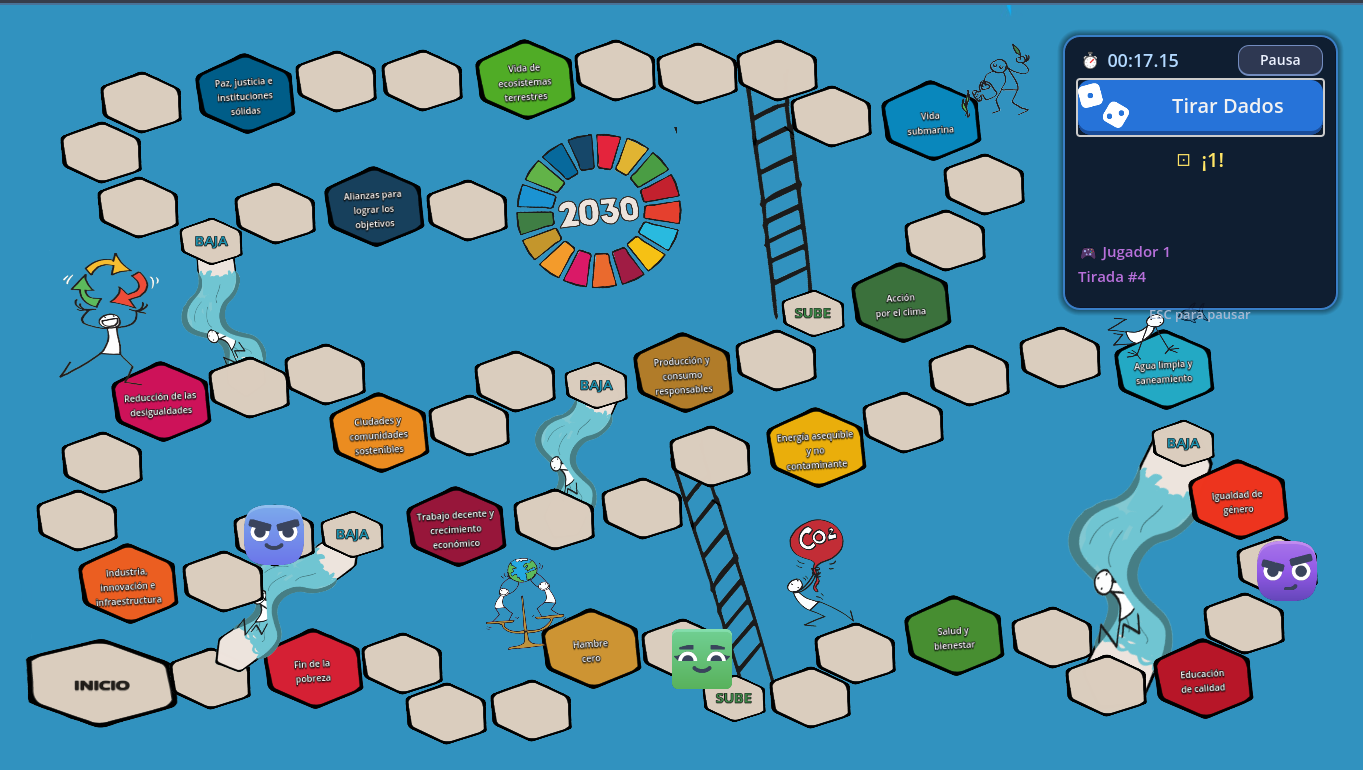
\includegraphics[width=0.7\textwidth]{Images/GoGoals Digital}
  \caption{Prototipo de la pantalla principal del tablero de juego (elaboración propia).\label{fig:prototipo_tablero}}
\end{figure}

\subsubsection{Panel de preguntas educativas}
\label{subsubsec:panel_preguntas}

El panel de preguntas constituye el componente central de la experiencia educativa del videojuego, ya que es el espacio donde se materializa la evaluación del conocimiento sobre los ODS. Este elemento funciona como una interfaz modal que se superpone al tablero durante las casillas temáticas, pausando temporalmente el flujo del juego para concentrar la atención del jugador en el contenido pedagógico. Su diseño responde a la necesidad de crear un momento de reflexión y aprendizaje dentro de la dinámica lúdica, equilibrando la competencia con la adquisición de conocimientos.

Tras la selección de una respuesta, el panel transita a un estado de retroalimentación que muestra un indicador visual claro (verde para correcto, rojo para incorrecto) acompañado de una breve explicación pedagógica que refuerza el aprendizaje. Esta retroalimentación permanece visible durante aproximadamente 5 segundos antes de cerrar el panel y continuar el turno, permitiendo que el jugador asimile la información sin interrumpir excesivamente el ritmo del juego.

\begin{figure}[H]
  \centering
  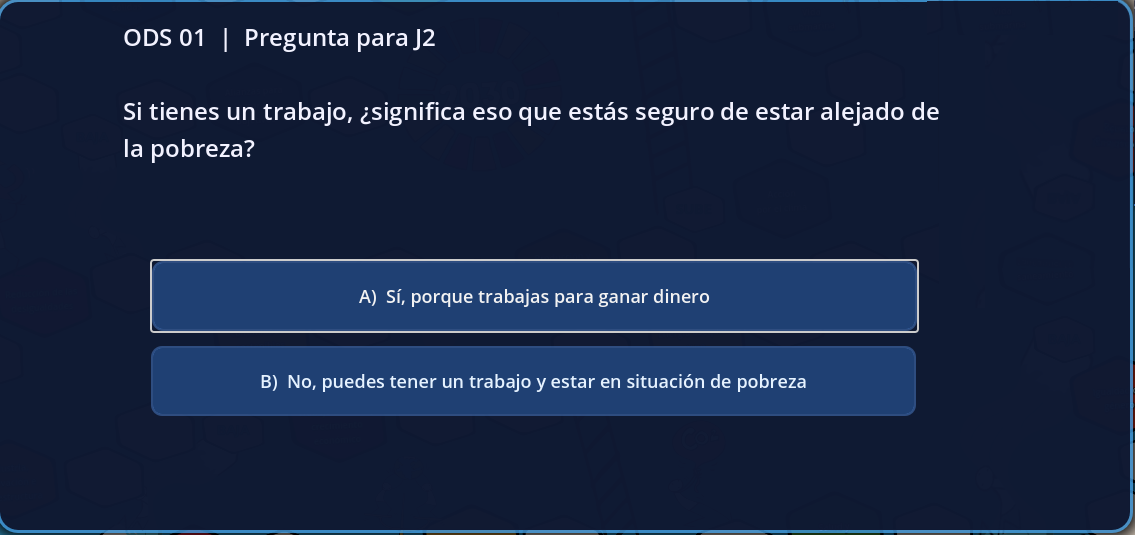
\includegraphics[width=0.75\textwidth]{Images/Panel Preguntas}
  \caption{Prototipo del panel de preguntas educativas por ODS (elaboración propia).\label{fig:prototipo_preguntas}}
\end{figure}

\subsubsection{Pantalla de estadísticas}
\label{subsubsec:pantalla_estadisticas}

La pantalla de estadísticas se presenta al finalizar la partida y constituye uno de los elementos más importantes desde el punto de vista pedagógico del videojuego. Esta interfaz muestra una tabla de clasificación ordenada que permite visualizar el desempeño comparativo de todos los jugadores participantes. La tabla presenta información estructurada en columnas que incluyen la posición final de cada jugador, el número de turnos que necesitó para completar el recorrido, el tiempo total invertido en la partida y el nombre del participante.

El criterio principal de ordenamiento es el número de turnos, considerando que un menor número de turnos indica un mejor desempeño en el conocimiento de los ODS, ya que implica menos retrocesos por respuestas incorrectas. En caso de empate en el número de turnos, el sistema utiliza el tiempo como criterio de desempate, favoreciendo al jugador que completó el recorrido en menor tiempo. Esta mecánica de clasificación incentiva tanto la precisión en las respuestas como la agilidad en la toma de decisiones.

\begin{figure}[H]
  \centering
  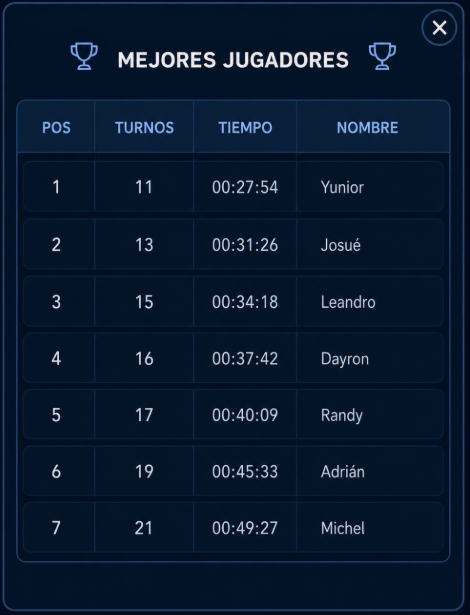
\includegraphics[width=0.35\textwidth]{Images/Ranking}
  \caption{Prototipo de la pantalla de estadísticas y clasificación final (elaboración propia).\label{fig:prototipo_estadisticas}}
\end{figure}

\subsection{Tarjetas CRC}
\label{subsec:tarjetas_crc}

Las tarjetas de clase, responsabilidad y colaboración constituyen una técnica fundamental en el diseño ágil, particularmente relevante en la metodología Extreme Programming. Son una herramienta efectiva para la conceptualización y diseño de sistemas orientados a objetos, que facilita la identificación de las clases, sus responsabilidades y las colaboraciones necesarias entre ellas \parencite{Sommerville2021}. A continuación se presenta, a modo ilustrativo, la tarjeta CRC del controlador principal del juego representado por la clase \texttt{GameManager} en la Tabla \ref{tab:crc_gamemanager}. El conjunto completo de las diez tarjetas CRC con el detalle arquitectónico restante se encuentra listado en el Anexo \ref{anx:tarjetas_crc}.

\begin{table}[H]
\centering
\caption{Tarjeta CRC GameManager (Controlador) (elaboración propia).\label{tab:crc_gamemanager}}
\begin{tabular}{|p{0.25\textwidth}|p{0.64\textwidth}|}
\hline
\multicolumn{2}{|c|}{\textbf{Tarjeta CRC}} \\
\hline
\textbf{Clase:} & GameManager \\
\hline
\textbf{Responsabilidades} & - orquestar el ciclo completo de la partida (inicio, turno, resolución de casilla, fin) \\
& - calcular rutas de movimiento e invocar animaciones \\
& - verificar condiciones de victoria \\
\hline
\textbf{Clases relacionadas} & GameState \\
& GameEvents \\
& BoardConfig \\
& AudioManager \\
\hline
\end{tabular}
\end{table}

La separación de responsabilidades reflejada en la tarjeta CRC de \texttt{GameManager} responde a una decisión concreta de diseño: centralizar el flujo evita que la lógica del turno quede dispersa en múltiples nodos de la interfaz, lo que generaría un acoplamiento implícito difícil de rastrear. Al delegar en \texttt{GameEvents} la notificación de cambios a la UI y en \texttt{GameState} la gestión del estado, el \texttt{GameManager} se mantiene cohesivo y reemplazable: cualquier componente de la interfaz que deba reaccionar a un evento de juego lo hace suscribiéndose a una se\~nal global, sin crear una dependencia directa con el controlador. Esta arquitectura elimina el acoplamiento temporal entre la lógica y la presentación, y simplifica las pruebas al poder invocar el controlador sin necesidad de instanciar la interfaz completa.



%---------------------------------------------------------------------------
\section{Implementación}
\label{sec:implementacion}

El presente epígrafe describe el proceso de implementación del videojuego educativo \textit{Go Goals! Digital}, abordando los estándares de codificación adoptados, los patrones de diseño aplicados y las tareas de ingeniería ejecutadas en cada iteración.

\subsection{Estándares de codificación}
\label{subsec:estandares}

Los estándares de codificación son un conjunto de convenciones y reglas que guían la forma en que se escribe el código fuente de un sistema, con el objetivo de mejorar su legibilidad, mantenibilidad y consistencia. Según \citeauthor{Sommerville2021} \parencite{Sommerville2021}, el cumplimiento de estándares de codificación es un factor clave para reducir la deuda técnica y facilitar la colaboración en equipos de desarrollo.

\subsubsection{Nomenclatura y estructura de archivos}
\label{subsubsec:nomenclatura}

Para el desarrollo en GDScript se aplicaron los siguientes estándares de nomenclatura, coherentes con las convenciones oficiales de la documentación de Godot \parencite{GodotDocs2026}. Estas convenciones facilitan la legibilidad del código y permiten que cualquier desarrollador familiarizado con Godot pueda comprender rápidamente la estructura del proyecto:

\begin{itemize}
    \item \textbf{Clases}: PascalCase, por ejemplo \texttt{GameManager} y \texttt{QuestionManager}.
    \item \textbf{Variables y funciones}: snake\_case, como \texttt{current\_player} y \texttt{roll\_dice()}.
    \item \textbf{Constantes}: SCREAMING\_SNAKE\_CASE, tales como \texttt{MAX\_PLAYERS} y \texttt{BOARD\_SIZE}.
    \item \textbf{Señales}: snake\_case prefijadas con el evento, por ejemplo \texttt{dice\_rolled} y \texttt{answer\_checked}.
    \item \textbf{Escenas}: PascalCase coincidiendo con el nombre de su script raíz, como \texttt{GameBoard.tscn}.
\end{itemize}

La arquitectura de directorios del proyecto obedece a una distribución basada en características funcionales, enfoque metodológico que agrupa componentes afines en espacios de trabajo claramente delimitados. En lugar de consolidar archivos únicamente por su formato u origen, el árbol segmenta los recursos en tres ramas principales. Primeramente, el directorio \texttt{assets} se encarga de aislar la multimedia estática transversal, albergando módulos de audio, fuentes tipográficas y elementos gráficos del tablero tales como los tokens o los tipos de hexágonos. Seguidamente, el bloque de \texttt{escenas} aloja las vistas empaquetadas instanciables, ilustradas por pantallas clave estilo \texttt{GameBoard} o \texttt{QuizView}. Por último, el núcleo lógico se aísla en la rama \texttt{scripts}, subdividida internamente en \texttt{clases} de entidad y componentes \texttt{singletons} de acceso global. Esta estricta separación semántica mitiga los tiempos de búsqueda, protege frente a la ruptura conflictiva de referencias internas propias del motor, y facilita que la escalabilidad a largo plazo del código base se sostenga de forma limpia y disciplinada:

\begin{figure}[H]
  \centering
  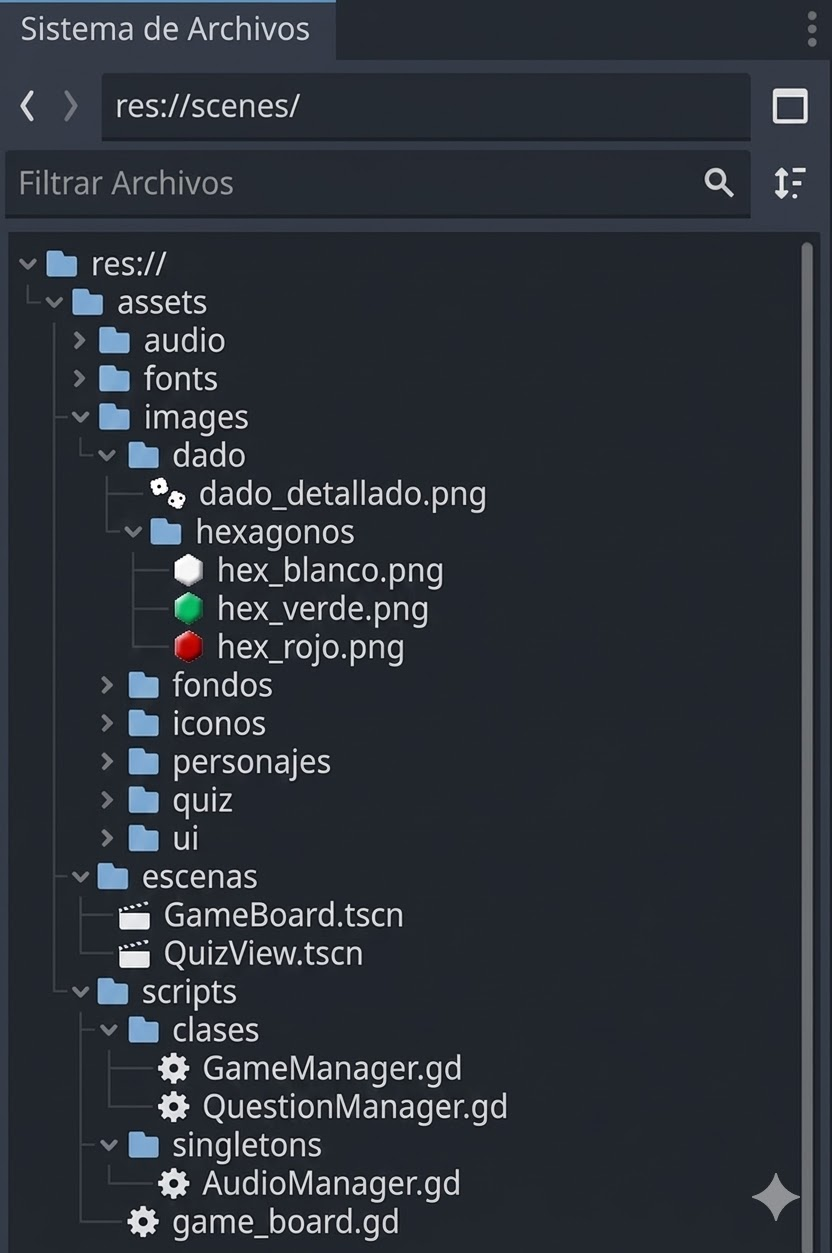
\includegraphics[width=0.35\textwidth]{Images/Jerarquia}
  \caption{Estructura de archivos del proyecto \textit{Go Goals! Digital} (elaboración propia).\label{fig:estructura_archivos}}
\end{figure}

\subsubsection{Documentación del código}
\label{subsubsec:documentacion_codigo}

Cada clase implementada en GDScript incluye comentarios de documentación al inicio del archivo describiendo su propósito, y comentarios de bloque en funciones de lógica compleja. Esta práctica facilita el mantenimiento futuro del código y permite la incorporación de nuevos desarrolladores al proyecto \parencite{GodotDocs2026}.

\subsection{Patrones de diseño utilizados}
\label{subsec:patrones}

Los patrones de diseño son soluciones reutilizables a problemas recurrentes en el desarrollo de software. Estos patrones proporcionan una manera estandarizada de abordar tareas de diseño recurrentes, mejorando la eficiencia y la coherencia del código. Al emplear patrones de diseño, los desarrolladores pueden beneficiarse de soluciones probadas que facilitan la comunicación, el mantenimiento y la extensibilidad del software \parencite{Pressman2019}. \textit{Go Goals! Digital} aplica los siguientes patrones de diseño, reflejados directamente en la estructura del código fuente.

\subsubsection{Patrones GRASP}
\label{subsubsec:patrones_grasp}

Son un conjunto de principios para asignar responsabilidades y funciones en el diseño de software orientado a objetos. Estos patrones ayudan a los desarrolladores a tomar decisiones coherentes sobre dónde ubicar la funcionalidad dentro del sistema. Al aplicar estos principios, se puede lograr un diseño de software más modular, flexible y fácil de mantener \parencite{Pressman2019}.

\textbf{Controlador de Fachada}

Tiene como objetivo asignar la responsabilidad de manejar las solicitudes del usuario a un componente específico, llamado controlador. En el proyecto, el script \texttt{GameManager.gd} centraliza la orquestación del ciclo de juego, delegando las tareas a otros objetos según sea necesario y coordinando el flujo general de la partida.

\textbf{Experto en información}

Se centra en asignar responsabilidades a la clase que posee la mayor cantidad de información necesaria para cumplir con dicha responsabilidad. Los modelos del proyecto, específicamente \texttt{Board.gd}, \texttt{Player.gd} y \texttt{Tile.gd}, encapsulan sus propias propiedades y aplican este principio, asegurando que cada entidad gestione únicamente sus propios datos.

\textbf{Bajo acoplamiento}

Este principio busca minimizar las dependencias entre las clases, lo que reduce el impacto de los cambios. Es notable que la configuración estática del tablero se aísla en \texttt{BoardConfig.gd}, separando los datos (escaleras, toboganes y casillas de quiz) de la lógica. Esta decisión de diseño garantiza que el sistema sea fácilmente extensible ante futuras modificaciones del tablero o las reglas del juego sin alterar el controlador principal.

\subsubsection{Patrones GOF}
\label{subsubsec:patrones_gof}

Los patrones de diseño GOF (Gang of Four) actúan como directrices estructuradas y probadas que brindan a los desarrolladores un marco sólido para abordar desafíos específicos organizados en categorías como creacionales, estructurales y de comportamiento.

\textbf{Singleton}

Garantiza que una clase tenga una única instancia y proporciona un punto de acceso global a ella. Godot implementa este patrón de forma nativa mediante el mecanismo de Autoloads. Los Autoloads del proyecto son \texttt{GameData} (repositorio central), \texttt{AudioManager} (gestión de sonido global) y \texttt{RecordsManager} (persistencia de datos), permitiendo que cualquier nodo acceda a estos servicios sin dependencias cruzadas \parencite{GodotDocs2026}.

\textbf{Observer (Bus de Eventos)}

Define una dependencia de uno-a-muchos entre objetos. El archivo \texttt{GameEvents} implementa una variante de este patrón a nivel de bus de eventos global. En lugar de conectar directamente un emisor con sus suscriptores, define se\~nales globales como \texttt{dice\_rolled} y \texttt{quiz\_requested} que cualquier componente emite o escucha de forma independiente, eliminando el acoplamiento entre el controlador y los componentes de la interfaz gráfica de usuario.

\begin{figure}[H]
  \centering
  \makebox[\textwidth]{\includegraphics[width=1.1\textwidth]{Images/signals}}
  \caption{Patrón Observer implementado mediante señales globales en Godot (elaboración propia).\label{fig:senales_godot}}
\end{figure}

\textbf{State (Máquina de Estados)}

Permite a un objeto alterar su comportamiento cuando su estado interno cambia. La alternativa más simple habría sido gestionar el estado de la partida mediante variables booleanas independientes, como \texttt{is\_paused}, \texttt{is\_rolling} e \texttt{is\_answering}. Sin embargo, este enfoque introduce de inmediato un problema estructural: las combinaciones de banderas pueden coexistir en estados inválidos, por ejemplo permitiendo que \texttt{is\_rolling = true} e \texttt{is\_answering = true} ocurran simultáneamente, generando condiciones de carrera y sentencias \texttt{if/else} anidadas que se vuelven inmanejables a medida que crece el sistema. El patrón \textit{State}, implementado en \texttt{GameState.gd} mediante una enumeración explícita de fases que abarca \texttt{MENU}, \texttt{PLAYING}, \texttt{PAUSED} y \texttt{GAME\_OVER}, garantiza que el sistema se encuentre en un único estado válido en cada instante. Las transiciones son atómicas y verificables, lo que simplifica la depuración, facilita las operaciones de guardado y restauración de estado y hace que el comportamiento del sistema sea predecible ante cualquier secuencia de eventos.

\subsubsection{Manejo de datos y persistencia}
\label{subsubsec:manejo_datos}

La arquitectura del videojuego exige un manejo robusto de los datos, separando la configuración persistente del estado efímero de la partida. Para ello, el Singleton \texttt{GameData} actúa como repositorio en memoria, mientras que \texttt{RecordsManager} se encarga de serializar y almacenar localmente las estadísticas de los jugadores en el sistema de archivos del usuario. El contenido pedagógico, que incluye el banco de preguntas por cada ODS, se almacena externamente en formato JSON, permitiendo actualizar el cuestionario sin necesidad de recompilar el proyecto.

El sistema implementa manejo de excepciones en los puntos críticos de entrada de datos. Ante la ausencia o invalidez sintáctica del archivo \texttt{questions.json}, se interrumpe la ejecución y se despliega una alerta: \textit{«Questions file not found or invalid. Please verify that \texttt{questions.json} exists in the data directory.»} Esta detención es intencional: el núcleo pedagógico del videojuego depende del banco de preguntas, por lo que carece de sentido continuar sin él. La validación semántica de cada pregunta se delega al redactor del archivo JSON, no al motor de juego, dado que el banco está diseñado para ser editado por educadores sin intervención del compilador.

\subsection{Tareas de ingeniería}
\label{subsec:tareas_ingenieria}

Las tareas de ingeniería son los componentes técnicos específicos derivados de las historias de usuario. Representan el trabajo concreto que debe realizarse para implementar cada funcionalidad. A continuación se expone de manera representativa, en la Tabla \ref{tab:ti5}, la tarea de ingeniería responsable del manejo interactivo de los ODS, vinculada a las HU9 y HU10 explicadas anteriormente. El conjunto completo con las diez tareas de ingeniería organizadas por iteración se encuentra disponible en el Anexo \ref{anx:tareas_ingenieria}.

\begin{table}[H]
\centering
\caption{Tarea de ingeniería 5: Sistema de preguntas y evaluación de respuestas (elaboración propia).\label{tab:ti5}}
\begin{tabular}{|p{0.3\textwidth}|p{0.65\textwidth}|}
\hline
\textbf{Campo} & \textbf{Descripción} \\
\hline
Tarea \# & 5 \\
\hline
HU relacionada & HU \#9, HU \#10 \\
\hline
Nombre & Implementación del sistema de preguntas y retroalimentación \\
\hline
Tipo & Desarrollo \\
\hline
Puntos estimados & 8.0 días \\
\hline
Iteración & 3 \\
\hline
Programador & Ruslan Alexei Martinez Campos \\
\hline
Descripción & Se integra el motor de lectura JSON para cargar preguntas ODS y se programa el panel modal interactivo para evaluar y retroalimentar al jugador. \\
\hline
\end{tabular}
\end{table}



%---------------------------------------------------------------------------
\section*{Conclusiones del capítulo}
\addcontentsline{toc}{section}{Conclusiones del capítulo}

El diseño del sistema a partir de los requisitos funcionales y no funcionales, plasmados en 18 historias de usuario y organizados en 5 iteraciones ágiles, confirmó la pertinencia de la metodología Extreme Programming para proyectos de software educativo de pequeña escala, al garantizar entregas incrementales y adaptación continua a las prioridades del cliente.

La arquitectura jerárquica basada en nodos de Godot, coordinada mediante servicios globales y un bus de eventos desacoplado, resultó la elección más adecuada para el proyecto por favorecer la extensibilidad de mecánicas y la mantenibilidad del código, al tiempo que la aplicación de los patrones GRASP y GoF (Singleton, Observer y State) aportó soluciones técnicas probadas a los problemas de gestión de estado, comunicación entre componentes y persistencia de datos.

La implementación de las diez tareas de ingeniería, bajo los estándares de codificación GDScript y con contenido educativo externalizado en formato JSON con validación de integridad, produjo un videojuego educativo funcional, de bajo peso, multiplataforma y con mecanismos de robustez ante errores en los datos, cumpliendo así con el objetivo propuesto en la investigación.

